% !TEX root = ../my-thesis.tex
%
\chapter{Appendix}
\label{sec:appendix}
\section{Probability Distributions}
\subsection{The Negative Binomial Distribution}
The negative binomial distribution is a univariate probability distribution that belongs to the discrete probability distributions. It models the number of trials required to achieve a given number of successes in a Bernoulli process. \\
The density is given by
\begin{equation}
    f\left(k,r,p\right)=\mathcal{P}\left(X=k\right)=\begin{pmatrix} k+r-1\\r-1\end{pmatrix}\left(1-p\right)^kp^r,
\end{equation}
with $r$ the number of successes, $k$ the number of failures, and $p$ the probability of success \cite{haldane1941fitting}.
\clearpage
\section{Distribution Fits}
\subsection{Distribution Fits for Germany}
% \begin{figure}[H]
%     \centering
%     \includesvg[width = 0.8\textwidth]{fit_normal_germany.svg}
%     \caption{A normal fit to the number of cases in German municipalities}
%     \label{fitNormalGermany}
% \end{figure}
\begin{figure}[H]
    \centering
    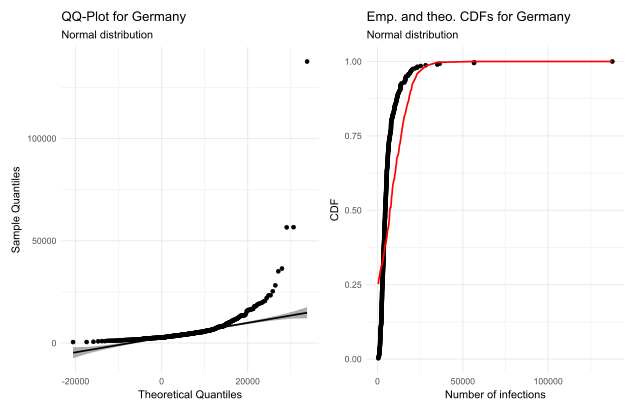
\includegraphics[width = 0.8\textwidth]{fit_normal_germany.png}
    \caption{A normal fit to the number of cases in German municipalities}
    \label{fitNormalGermany}
\end{figure}
% \begin{figure}[H]
%     \centering
%     \includesvg[width = 0.8\textwidth]{fit_poisson_germany.svg}
%     \caption{A Poisson fit to the number of cases in German municipalities}
%     \label{fitPoissonGermany}
% \end{figure}
\begin{figure}[H]
    \centering
    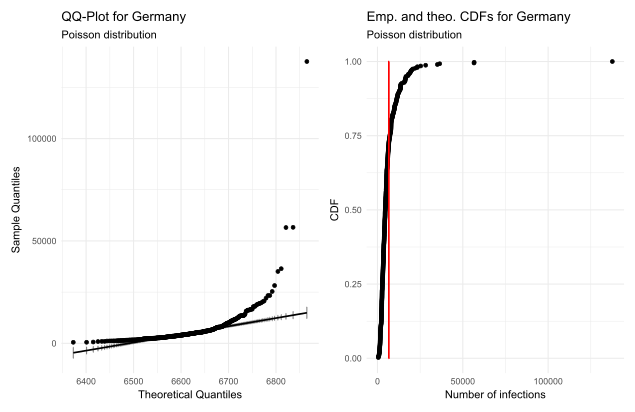
\includegraphics[width = 0.8\textwidth]{fit_poisson_germany.png}
    \caption{A Poisson fit to the number of cases in German municipalities}
    \label{fitPoissonGermany}
\end{figure}
\subsection{Distribution Fits for Norway}
% \begin{figure}[H]
%     \centering
%     \includesvg[width = 0.8\textwidth]{fit_normal_norway.svg}
%     \caption{A normal fit to the number of cases in Norwegian municipalities}
%     \label{fitNormalNorway
% \end{figure}
\begin{figure}[H]
    \centering
    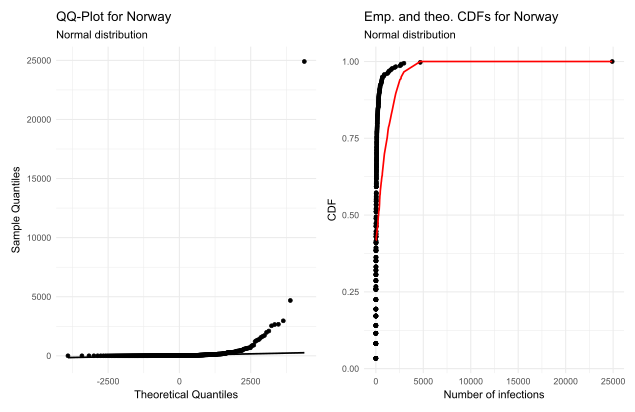
\includegraphics[width = 0.8\textwidth]{fit_normal_norway.png}
    \caption{A normal fit to the number of cases in Norwegian municipalities}
    \label{fitNormalNorway}
\end{figure}
% \begin{figure}[H]
%     \centering
%     \includesvg[width = 0.8\textwidth]{fit_poisson_norway.svg}
%     \caption{A Poisson fit to the number of cases in Norwegian municipalities}
%     \label{fitPoissonNorway}
% \end{figure}
\begin{figure}[H]
    \centering
    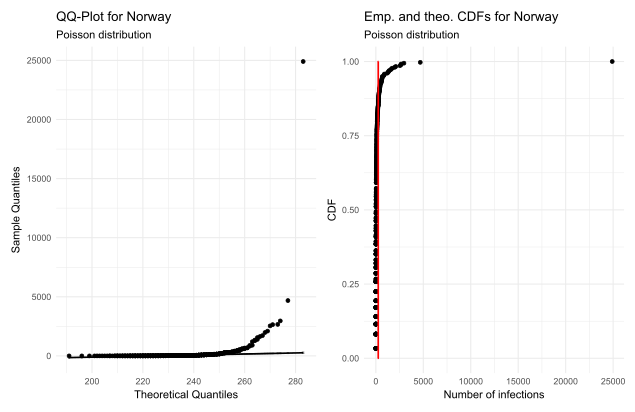
\includegraphics[width = 0.8\textwidth]{fit_poisson_norway.png}
    \caption{A Poisson fit to the number of cases in Norwegian municipalities}
    \label{fitPoissonNorway}
\end{figure}
\clearpage
\section{Code examples}
\subsection{Specifying the Different Types of Models}
\begin{lstlisting}[caption={Specifying different models in INLA.}, label={codeModels}, language=R]
# set the seed
set.seed(420)
# draw a sample
test <- sample(
    seq_len(nrow(newest_numbers)),
    size = floor(0.2 * nrow(newest_numbers))
  )
# get the number of infections for the test data
test_value <- newest_numbers$value[test]
# set the number of infections to NA in the train data
newest_numbers$value[test] <- NA
# define the link function
link <- rep(NA, nrow(newest_numbers))
link[which(is.na(newest_numbers$value))] <- 1
# define the penalised prior
prior_1 <- list(
  prec = list(
    prior = "pc.prec",
    param = c(1, 0.01)
  )
)
# create the neighbordhood matrix
nb <- poly2nb(newest_numbers)
# save the matrix
nb2INLA("maps/map.adj", nb)
g <- inla.read.graph(filename = "maps/map.adj")
# define the C matrix for the Leroux model
Q <- Diagonal(x = sapply(nb, length))
for (i in 2:nrow(newest_numbers)) {
  Q[i - 1, i] <- -1
  Q[i, i - 1] <- -1
}

C <- Diagonal(x = 1, n = nrow(newest_numbers)) - Q
# define the formula for besags proper model
formula_besag <- value ~
  pop_dens + urb_dens + sex +
  f(idarea_1, model = "besagproper", graph = g, hyper = prior_1)
# define the formula for bym2 model
formula_bym2 <- value ~
  pop_dens + urb_dens + sex +
  f(
    idarea_1, model = "bym2", graph = g,
    scale.model = TRUE, hyper = prior_1
  )
# define the formula for leroux model
formula_leroux <- value ~
  pop_dens + urb_dens + sex +
  f(idarea_1, model = "generic1", Cmatrix = C, hyper = prior_1)
# compute the models
res_besag <- inla(
  formula_besag,
  family = "nbinomial",
  data = newest_numbers,
  E = expected_count,
  control.predictor = list(
    compute = TRUE,
    link = link
  ),
  Ntrials = newest_numbers$population,
  control.compute = list(dic = TRUE, waic = TRUE, cpo = TRUE)
)
res_bym2 <- inla(
  formula_bym2,
  family = "nbinomial",
  data = newest_numbers,
  E = expected_count,
  control.predictor = list(
    compute = TRUE,
    link = link
  ),
  Ntrials = newest_numbers$population,
  control.compute = list(dic = TRUE, waic = TRUE, cpo = TRUE)
)
res_leroux <- inla(
  formula_leroux,
  family = "nbinomial",
  data = newest_numbers,
  E = expected_count,
  control.predictor = list(
    compute = TRUE,
    link = link
  ),
  Ntrials = newest_numbers$population,
  control.compute = list(dic = TRUE, waic = TRUE, cpo = TRUE)
)
\end{lstlisting}
\subsection{Making Predictions for the Test Data}
\begin{lstlisting}[caption={The code for making predictions in INLA.}, label={codePrediction}, language=R]
# create a vector to save the predictions to
predicted <- c()
# now make the predictions
for(i in seq_len(nrow(newest_numbers))) {
  predicted[i] <- inla.emarginal(
    function(x) x * newest_numbers$population[i],
    res_bym2$marginals.fitted.values[[i]]
  )
}
# calculate the MAE for the test data
mean(abs(predicted[test] - test))

\end{lstlisting}
\subsection{Variable Selection using INLA}
\begin{lstlisting}[caption={The code for variable selection in INLA.}, label={codeSelection}, language=R]
# define the stack
stack_all <- inla.stack(
  data = list(value = newest_numbers$value),
  A = list(1),
  effects = list(
    data.frame(
      Intercept = 1,
      newest_numbers[, c(2:15, 20:35, 43:46)]
    )
  )
)
# run backwards varaible selection
result_all_backwards <- INLAstep(
  fam1 = "nbinomial",
  newest_numbers,
  in_stack = stack_all,
  invariant = "Intercept",
  direction = "backwards",
  include = c(2:15, 20:35, 43:46),
  y = "value",
  y2 = "value",
  powerl = 1,
  inter = 1,
  thresh = 2,
  num.threads = 7
)
# run forwards variable selection
result_all_forwards <- INLAstep(
  fam1 = "nbinomial",
  newest_numbers,
  in_stack = stack_all,
  invariant = "Intercept",
  direction = "forwards",
  include = c(2:15, 20:35, 43:46),
  y = "value",
  y2 = "value",
  powerl = 1,
  inter = 1,
  thresh = 2,
  num.threads = 7
)
\end{lstlisting}
\subsection{Calculating the Posterior Mean}
\begin{lstlisting}[caption={Calculating the posterior mean of a coefficent.}, label={codePosteriorMean}, language=R]
inla.emarginal(exp, model_leroux$marginals.fixed$trade_tax)
# calculate the increase in risk for an increase 
# by 2 in the trade tax
inla.emarginal(
  exp,
  model_leroux$marginals.fixed$trade_tax
  ) ^ 2
\end{lstlisting}
\subsection{Calculating a Credibility Interval}
\begin{lstlisting}[caption={Extracting the credibility interval for a coefficient}, label={codeCredibility}, language=R]
inla.qmarginal(
  c(0.025,0.975),
  inla.tmarginal(
    exp,
    model_leroux$marginals.fixed$trade_tax
  )
)
\end{lstlisting}
\subsection{Best Spatial Models For Germany}
\subsubsection{Best Spatial Model using Demographic Variables}
\begin{lstlisting}[caption={The code for the demographic models.}, label={codeDemoGermany}, language=R]
prior_2 <- list(
  prec = list(
    prior = "pc.prec",
    param = c(0.5 / 0.31, 0.01)
  )
)
formula <- value ~
  Union + SPD + Gruene + FDP +
  die_linke + afd + 
  f(idarea_1, model = "generic1", Cmatrix = C, hyper = prior_2)
\end{lstlisting}
\subsubsection{Best Spatial Model using Infrastructural Variables}
\begin{lstlisting}[caption={The code for the demographic models.}, label={codeInfraGermany}, language=R]
prior_1 <- list(
  prec = list(
    prior = "pc.prec",
    param = c(1, 0.01)
  )
)
formula <- value ~
  marketplace + entertainment + sport + clinic +
  hairdresser + shops + place_of_worship + retail + nursing_home +
  restaurant + aerodrome + office + platform + schools +
  higher_education + kindergarten + bakeries + 
  f(
    idarea_1, model = "bym2", graph = G,
    scale.model = TRUE, hyper = prior_1
  )
\end{lstlisting}
\subsubsection{Best Spatial Model using Both Types of Variables}
\begin{lstlisting}[caption={The code for the demographic models.}, label={codeBothGermany}, language=R]
prior_1 <- list(
  prec = list(
    prior = "pc.prec",
    param = c(1, 0.01)
  )
)
formula <- value ~
  schools + afd + die_linke + pop_dens +
  place_of_worship + entertainment + bakeries + SPD +
  platform + sport + nursing_home + welfare_recipients +
  FDP + kindergarten + log(trade_tax) + office +
  f(
    idarea_1, model = "bym2", graph = g,
    scale.model = TRUE, hyper = prior_1
  )
\end{lstlisting}
\subsection{Best Spatial Models For Norway}

\clearpage
\section{Models}
\subsubsection{Coefficients of BYM2 Model with all Variables for Germany}
\begin{table}[H] 
\caption{The fixed effects for the BYM2 model. Values are rounded. \label{allGermanyBYM2}}
\begin{tabular}{l r r r r}
\toprule
\textbf{Variable}	& \textbf{Mean}	& \textbf{exp(mean$_{\hbox{p}}$)} & \textbf{exp(q0025$_{\hbox{p}}$)} & \textbf{exp(q0975$_{\hbox{p}}$)} \\
\midrule
(Intercept) & -2.752 & 0.1308 & 0.005269 & 0.6603\\
AfD & 3.930 & 57.70  & 19.04 & 135.1 \\
sex & 3.726 & 436.4 & -528.5 & 2156 \\
Union & 0.8027 & 2.406 & 1.044 & 4.758 \\
aerodrome & 0.3879 & 1.806 & 0.4220 & 5.111 \\
kindergarten & 0.1613 & 1.182 & 0.9437 & 1.463 \\
entertainment & 0.1275 & 1.211 & 0.5643 & 2.282 \\
shops & 0.06951 & 1.084 & 0.7961 & 1.442 \\
nursing\_home & 0.06812 & 1.144 & 0.5251 & 2.175 \\
bakeries & 0.05613 & 1.068 & 0.8035 & 1.392 \\
sport & 0.04839 & 1.052 &  0.9203 & 1.120 \\
unemployed\_ & \multirow{2}{*}{0.04093} & \multirow{2}{*}{1.042}  & \multirow{2}{*}{1.026} & \multirow{2}{*}{1.057}\\
foreigners  \\
asylum\_seeker\_ & \multirow{2}{*}{0.004844} & \multirow{2}{*}{1.005}  & \multirow{2}{*}{0.9950} & \multirow{2}{*}{1.015}\\
benefits  \\
pop\_dens & 0.00007097 & 1.000 & 1.000 & 1.000 \\
total\_income & 0.00001266 & 1.000 & 1.000 & 1.000 \\
urb\_dens & 0.000009849  & 1.0000 & 0.9993 & 1.001 \\
trade\_tax &  0.0000001765 & 1.0000 & 1.000 & 1.000\\
income\_tax &  -0.00006125 & 0.9999 &  0.9998 & 1.000 \\
welfare\_ & \multirow{2}{*}{-0.001508} & \multirow{2}{*}{0.9985}  & \multirow{2}{*}{0.9852} & \multirow{2}{*}{1.012}\\
recipients \\
protection\_ & \multirow{2}{*}{-0.003726} & \multirow{2}{*}{0.9963}  & \multirow{2}{*}{0.9926} & \multirow{2}{*}{1.000}\\
seekers \\
unemployed\_ & \multirow{2}{*}{-0.008041} & \multirow{2}{*}{0.9920}  & \multirow{2}{*}{0.9857} & \multirow{2}{*}{0.9984} \\
total \\
platform & -0.008767  & 0.9913 &  0.9821 & 1.000 \\
schools & -0.01115  & 0.9935 & 0.8194 & 1.193 \\
FDP & -0.01648  & 2.490 & 0.04743 & 14.02\\
restaurant & -0.03560  & 0.9654 & 0.9113 & 1.022 \\
clinic & -0.03697  & 0.9646 &  0.8853 & 1.049 \\
hairdresser & -0.05900  & 0.9483 & 0.7617 & 1.1166 \\
SPD & -0.1807  & 0.9439 & 0.3160 & 2.197 \\
die\_linke & -0.2930  & 1.043 &  0.1483 & 3.682 \\
other\_parties & -12.22  & 1.469e+31 & -8.710e+8 & 1.468e+04\\
\bottomrule
\end{tabular}
\end{table}